% Copyright 2026 Sreeram Anil
% SPDX-License-Identifier: CC-BY-4.0
\chapter{Dual sigma-point Kalman filter (Dual SPKF)}
\label{ch:dualukf}

\section*{At a glance}
\begin{tabular}{@{}l>{\raggedright\arraybackslash}p{0.76\textwidth}@{}}
Family & Joint/dual state--parameter estimation (SOH) \\
Header & \texttt{include/estkit/parameter/dual\_ukf.hpp} \\
Registered name & \texttt{DualUKF} \\
State dimension & two filters: $n_x=4$ ($9$ sigma points) and $n_p=2$ ($5$ sigma points) \\
Cost per step & $\mathcal{O}(n_x^3+n_p^3)$, $9+5$ model evaluations; \SI{2.38}{\micro\second}/step measured \\
Primary references & \cite{plett2006spkf2,wannelson2001dual,plett2004ekf3,julier2004unscented} \\
\end{tabular}

\section{Motivation and aerospace/BMS relevance}
The dual SPKF combines the two ideas of the preceding chapters: the decoupling of the state and
parameter filters (Chapter~\ref{ch:dualekf}), which lets the parameter tracking rate be tuned
independently and keeps the cost at $n_x^3+n_p^3$, and the derivative-free sigma-point propagation
(Chapter~\ref{ch:jointukf}), which handles the bilinear $i/Q$ and $R_0 i$ terms without a Jacobian.
Plett describes it in Part~2 of the sigma-point series~\cite{plett2006spkf2} as the
lower-cost alternative to the joint SPKF for packs with many cells, where the augmented state of a
joint filter becomes unmanageable.

It is also the most delicate member of the family, and the reason is worth stating up front because
it drives the whole implementation.  The parameter filter's ``measurement function'' is the output
that the \emph{state filter} would predict if the parameters were $\vtheta$.  Evaluating that
function with a single, shared state estimate --- the obvious reading of the algorithm --- destroys
the very cancellation that makes the dual EKF stable (Remark~\ref{rem:de-r3}), because it reports
the one-step sensitivity $\partial h/\partial R_0=-\mathrm{arr}(T)\,i$ instead of the total
sensitivity, which is nearly zero.  On the ECM plant this is not a subtle degradation: the naive
version drives $R_0$ into its lower bound within \SI{1.2}{\second} and ends the mission with an SOC
RMSE of $0.10$ instead of $0.002$.  The fix, derived below, is to give every parameter sigma point
its own state replica.

\section{Problem statement and assumptions}
The plant, the random walk and the two-filter structure are those of Chapter~\ref{ch:dualekf}.  The
state filter is now a UKF, and the parameter filter is a sigma-point filter of dimension $n_p$ whose
measurement model is
\begin{equation}
\vy_k = d_k(\vtheta)+\bm{e}_k, \qquad
d_k(\vtheta)=h\!\left(f\!\left(\xplus_{k-1}(\vtheta),\vu_{k-1};\vtheta\right),\vu_k;\vtheta\right),
\label{eq:du-meas}
\end{equation}
where $\xplus_{k-1}(\vtheta)$ denotes the posterior state that the filter would hold at $k-1$ had it
been running with $\vtheta$ all along.

\begin{assumption}[Replica propagation]\label{as:du-rep}
$\xplus_{k-1}(\vtheta)$ is approximated, for each parameter sigma point, by a state replica
propagated with the sigma point's own parameters and corrected with the \emph{state filter's} gain,
Eq.~\eqref{eq:du-rep} below.  This is the sigma-point image of Assumption~\ref{as:de-gain}.
\end{assumption}

\begin{assumption}[Parameter-filter measurement noise]\label{as:du-R}
As in Chapter~\ref{ch:dualekf}, the residual driving the parameter filter contains the state
estimation error and the correlated part of the model error, so
$\mR_\theta=\gamma_\theta\left(\mR+\mH\mP^-_k\mH^\T\right)$ with a tuning factor
$\gamma_\theta\ge1$ (Plett tunes the parameter filter's $\bm{\Sigma}_e$ independently of the state
filter's~\cite[§5]{plett2006spkf2}).
\end{assumption}

\section{Derivation}

\subsection{Parameter sigma points}
Let $\bm{\mathcal{W}}^{(j)}$, $j=0,\dots,2n_p$, be the scaled unscented sigma set of
$\N{\hat{\vtheta}^-_k}{\bm{\Sigma}^-_{\theta,k}}$, built exactly as in \eqref{eq:ju-sigma} but with
$n_a$ replaced by $n_p$ and with its own scaling parameters
$(\alpha_\theta,\beta_\theta,\kappa_\theta)$.  Each $\bm{\mathcal{W}}^{(j)}$ is projected onto the
physical box before use.

\subsection{State replicas: the sigma-point total derivative}
Associate with every parameter sigma point a state replica $\hat{\vx}^{(j)}$, initialised to
$\vx_0$.  At each step,
\begin{align}
\hat{\vx}^{(j),-}_k &= f\!\left(\hat{\vx}^{(j),+}_{k-1},\vu_{k-1};\bm{\mathcal{W}}^{(j)}\right), &
d^{(j)}_k &= h\!\left(\hat{\vx}^{(j),-}_k,\vu_k;\bm{\mathcal{W}}^{(j)}\right),
\label{eq:du-prop}\\
\hat{\vx}^{(j),+}_k &= \hat{\vx}^{(j),-}_k+\mK_k\left(\vy_k-d^{(j)}_k\right). &&
\label{eq:du-rep}
\end{align}
Equation~\eqref{eq:du-rep} is the exact sigma-point analogue of Plett's
$\partial\xplus/\partial\vtheta=\partial\xminus/\partial\vtheta-\mK\,\partial\hat{y}/\partial\vtheta$,
Eq.~\eqref{eq:de-r3}: differentiating \eqref{eq:du-rep} with respect to $\vtheta$ and taking the
limit of small sigma spread reproduces it term by term.  Its effect is the cancellation of
Remark~\ref{rem:de-r3}: a replica whose $R_0$ is larger than the mean predicts a lower voltage, is
therefore pushed to a higher SOC by \eqref{eq:du-rep}, and at the next step predicts almost the same
voltage as the mean replica.  The spread of $d^{(j)}$ across the sigma set is then the \emph{total}
sensitivity, which is what the parameter filter must see.

Because $n_y=1$ here, the state filter's gain is never formed explicitly: from
$\mK_k\,\nu_k=\xplus_k-\xminus_k$ with $\nu_k$ the state filter's own innovation,
\begin{equation}
\mK_k\left(y_k-d^{(j)}_k\right)=\left(\xplus_k-\xminus_k\right)\frac{y_k-d^{(j)}_k}{\nu_k},
\qquad |\nu_k|>\epsilon ,
\label{eq:du-gainfree}
\end{equation}
which costs one scalar division.  After the update the replica bank is re-centred on the state
filter's estimate,
$\hat{\vx}^{(j),+}\leftarrow\hat{\vx}^{(j),+}+\left(\xplus_k-\tfrac{1}{2n_p+1}\sum_l\hat{\vx}^{(l),+}\right)$,
so that it can never drift away from the filter it is supposed to shadow.

\subsection{Parameter measurement update}
With $\hat{y}_k=\sum_j w^{(j)}_m d^{(j)}_k$,
\begin{align}
\mP_{dd}&=\sum_j w^{(j)}_c\left(d^{(j)}_k-\hat{y}_k\right)\left(\cdot\right)^\T+\mR_\theta, &
\mP_{\theta d}&=\sum_j w^{(j)}_c\left(\bm{\mathcal{W}}^{(j)}-\hat{\vtheta}^-_k\right)\left(d^{(j)}_k-\hat{y}_k\right)^\T,
\label{eq:du-mu}\\
\mL_{\theta,k}&=\mP_{\theta d}\mP_{dd}\inv, &
\hat{\vtheta}^+_k&=\hat{\vtheta}^-_k+\mL_{\theta,k}\left(\vy_k-\hat{y}_k\right),
\label{eq:du-upd}
\end{align}
\begin{equation}
\bm{\Sigma}^+_{\theta,k}=\bm{\Sigma}^-_{\theta,k}-\mL_{\theta,k}\mP_{dd}\mL_{\theta,k}^\T .
\label{eq:du-cov}
\end{equation}
The diagonal of $\bm{\Sigma}^+_\theta$ is floored at $\bm{\Sigma}_r$ so that round-off can never
make it non-positive.

\section{Algorithm}
\begin{algorithm}[H]
\caption{Dual SPKF --- one sampling period}
\begin{algorithmic}[1]
\Require $\xplus_{k-1},\mP^+_{k-1},\hat{\vtheta}^+_{k-1},\bm{\Sigma}^+_{\theta,k-1},\{\hat{\vx}^{(j),+}_{k-1}\},\vu_{k-1},\vy_k,\vu_k$
\State \textbf{Parameter time update:} $\bm{\Sigma}^-_\theta\gets\bm{\Sigma}^+_\theta+\bm{\Sigma}_r$; build $\{\bm{\mathcal{W}}^{(j)}\}$, project onto the box
\State \textbf{Replica time update:} $\hat{\vx}^{(j),-}_k\gets f(\hat{\vx}^{(j),+}_{k-1},\vu_{k-1};\bm{\mathcal{W}}^{(j)})$ for all $j$
\State \textbf{State time update:} unscented predict of the UKF with $\hat{\vtheta}^-_k$
\State \textbf{Parameter measurement update:} $d^{(j)}_k\gets h(\hat{\vx}^{(j),-}_k,\vu_k;\bm{\mathcal{W}}^{(j)})$; \eqref{eq:du-mu}--\eqref{eq:du-cov}; clamp $\hat{\vtheta}^+_k$
\State \textbf{State measurement update:} unscented update; record $\nu_k$ and $\xplus_k-\xminus_k$
\State \textbf{Replica measurement update:} \eqref{eq:du-rep} via \eqref{eq:du-gainfree}; constrain; re-centre
\State write $\hat{\vtheta}^+_k$ into the state filter's model
\Ensure $\xplus_k,\mP^+_k,\hat{\vtheta}^+_k,\bm{\Sigma}^+_{\theta,k},\{\hat{\vx}^{(j),+}_k\}$
\end{algorithmic}
\end{algorithm}

\section{Application to the battery model}
The state filter is \texttt{Ukf<EcmModel>} with the standard $\alpha=0.1$, $\beta=2$, $\kappa=0$.
The parameter filter uses $\alpha_\theta=1$, $\beta_\theta=2$, $\kappa_\theta=0$, so
$\lambda=0$, $c=n_p=2$, $w^{(0)}_m=0$ and $w^{(j)}=1/4$: the sigma points sit at
$\pm\sqrt{2}\,\sigma$, which is a well-spread and numerically safe choice for a two-dimensional,
nearly linear parameter subproblem.  The priors, the random walk and the boxes are identical to the
other three joint/dual filters (Section~\ref{sec:je-app}).

The one tuning knob that differs is $\gamma_\theta$ of Assumption~\ref{as:du-R}, set to $9$
(i.e.\ a $3\sigma$ inflation of the parameter filter's measurement standard deviation).  This is
not a cosmetic choice: the residual that drives \eqref{eq:du-upd} contains the state error and the
correlated ECM model error (unmodelled Preisach hysteresis, OCV-table interpolation, the truncation
of the RC ladder to two branches), none of which is white with the sensor's
$\sigma_v=\SI{2}{\milli\volt}$.  Measured on \texttt{aged\_cell}, raising $\gamma_\theta$ from $1$ to
$9$ takes the steady-state SOC RMSE from $0.0170$ to about $0.0013$ and the capacity error from
\SI{-0.154}{\ampere\hour} to \SI{+0.018}{\ampere\hour}; $\gamma_\theta=16$ was also tried and
degrades \texttt{sensor\_dropout}, so $9$ is used.  A \emph{fixed} inflation is the weak point of
this tuning: Chapter~\ref{ch:dualekf} shows that the same quantity estimated on-line from the
measured residual statistics adapts to plants and temperatures that a constant cannot.

The replica mechanism is exposed as \texttt{state\_replicas} (default on).  Turning it off
reproduces the naive one-step dual SPKF and is retained only so that the effect can be demonstrated:
with a shared state the nominal SOC RMSE is $0.102$ and $R_0$ saturates at its lower box bound.

\section{Implementation notes}
Storage is \SI{5512}{\byte}: the UKF, the $2\times2$ parameter covariances, five parameter sigma
points and ten state replicas ($5$ prior, $5$ posterior) of four components each.  No heap, no
exceptions.  The measured cost is \SI{2.38}{\micro\second}/step, half that of the joint SPKF,
because the two Cholesky factorisations are $4\times4$ and $2\times2$ instead of $6\times6$ and the
model is evaluated $9+5$ rather than $2\times13$ times.

Every parameter update is guarded: if $\mP_{dd}$ is singular or the update is not finite the
parameter step is skipped.  The replica correction \eqref{eq:du-gainfree} divides by the state
filter's innovation, which is floored at $10^{-12}$; when the innovation is that small the
correction is negligible anyway and the replicas simply take the same shift as the filter.

The main limitation is the one of every dual method: the parameter filter consumes the state
filter's residual and cannot distinguish model error from parameter error.  The
$\gamma_\theta$ inflation mitigates but does not remove it.

\section{Benchmark results}
\label{sec:du-results}
% Copyright 2026 Sreeram Anil
% SPDX-License-Identifier: CC-BY-4.0
\begin{table}[H]\centering\footnotesize\setlength{\tabcolsep}{4pt}
\caption{DualUKF: cell-level benchmark on the eVTOL mission (mean over seeds; RMSE and max error in \% SOC; $t_\mathrm{conv}$: first time the error stays below 2\,\% for 60\,s, -- = never; EKF reference: steady-state RMSE of the plain EKF on the same data).}\label{tab:cell_DualUKF}
\begin{tabular}{llrrrrrcrr}\toprule
plant & scenario & RMSE & RMSE$_\mathrm{ss}$ & max & $t_\mathrm{conv}$ [s] & RMSE$_v$ [mV] & div. & EKF ref. & ns/step \\ \midrule
ECM & nominal & 0.20 & 0.09 & 4.02 & 0 & 1.11 & no & 0.05 & 2371 \\
ECM & init\_error & 0.63 & 0.12 & 3.30 & 70 & 2.08 & no & 0.05 & 2377 \\
ECM & current\_bias & 0.69 & 0.71 & 3.84 & 0 & 1.09 & no & 0.61 & 2376 \\
ECM & noise\_step & 0.27 & 0.27 & 4.02 & 0 & 3.00 & no & 0.12 & 2370 \\
ECM & outliers & 0.82 & 0.77 & 4.92 & 5 & 2.29 & no & 0.21 & 2369 \\
ECM & cold & 1.38 & 1.61 & 4.03 & 1 & 2.47 & no & 0.16 & 2374 \\
ECM & hot & 0.14 & 0.04 & 4.03 & 0 & 0.92 & no & 0.03 & 2372 \\
ECM & aged\_cell & 0.27 & 0.11 & 4.36 & 0 & 1.34 & no & 1.52 & 2356 \\
ECM & param\_mismatch & 2.06 & 2.70 & 4.27 & 0 & 1.26 & no & 1.36 & 2369 \\
ECM & sensor\_dropout & 3.64 & 4.12 & 8.65 & 0 & 2.32 & no & 0.46 & 2370 \\
ECM & preisach & 1.88 & 1.28 & 6.19 & 224 & 1.23 & no & 0.20 & 2370 \\
ECM & combined & 1.87 & 2.10 & 7.70 & 0 & 2.44 & no & 12.44 & 2369 \\
\midrule
SPM & nominal & 4.41 & 3.68 & 6.46 & 0 & 1.17 & no & 3.73 & 2219 \\
SPM & init\_error & 3.50 & 1.74 & 6.58 & 1301 & 2.03 & no & 3.81 & 2211 \\
SPM & current\_bias & 5.62 & 5.59 & 6.82 & 0 & 1.18 & no & 5.69 & 2232 \\
SPM & noise\_step & 4.07 & 2.99 & 6.46 & 0 & 3.20 & no & 3.30 & 2206 \\
SPM & outliers & 4.44 & 4.63 & 8.50 & 13 & 2.54 & no & 1.99 & 2236 \\
SPM & cold & 8.17 & 6.59 & 11.09 & 607 & 2.59 & no & 7.35 & 2229 \\
SPM & hot & 1.57 & 0.86 & 4.41 & 0 & 0.94 & no & 2.16 & 2217 \\
SPM & param\_mismatch & 3.53 & 2.39 & 6.05 & 0 & 1.17 & no & 3.13 & 2215 \\
SPM & sensor\_dropout & 7.52 & 6.44 & 10.46 & 0 & 2.20 & no & 5.31 & 2247 \\
\bottomrule\end{tabular}\end{table}
\begin{table}[H]\centering\small\caption{DualUKF: additional outputs (capacity error at the end of the mission in Ah, averaged over the last 10\,\% of the run; interval-bound violation rate).}\label{tab:cellx_DualUKF}
\begin{tabular}{llrr}\toprule plant & scenario & $\hat Q - Q$ [Ah] & bound violation [\%] \\ \midrule
ECM & nominal & +0.029 & -- \\
ECM & init\_error & +0.030 & -- \\
ECM & current\_bias & +0.329 & -- \\
ECM & noise\_step & +0.020 & -- \\
ECM & outliers & -0.007 & -- \\
ECM & cold & +0.085 & -- \\
ECM & hot & +0.041 & -- \\
ECM & aged\_cell & +0.013 & -- \\
ECM & param\_mismatch & +0.324 & -- \\
ECM & sensor\_dropout & +0.512 & -- \\
ECM & preisach & +0.132 & -- \\
ECM & combined & +0.242 & -- \\
SPM & nominal & +0.906 & -- \\
SPM & init\_error & +0.976 & -- \\
SPM & current\_bias & +1.102 & -- \\
SPM & noise\_step & +1.132 & -- \\
SPM & outliers & +0.536 & -- \\
SPM & cold & +1.474 & -- \\
SPM & hot & +0.614 & -- \\
SPM & param\_mismatch & +1.170 & -- \\
SPM & sensor\_dropout & +1.384 & -- \\
\bottomrule\end{tabular}\end{table}

\begin{figure}[H]\centering
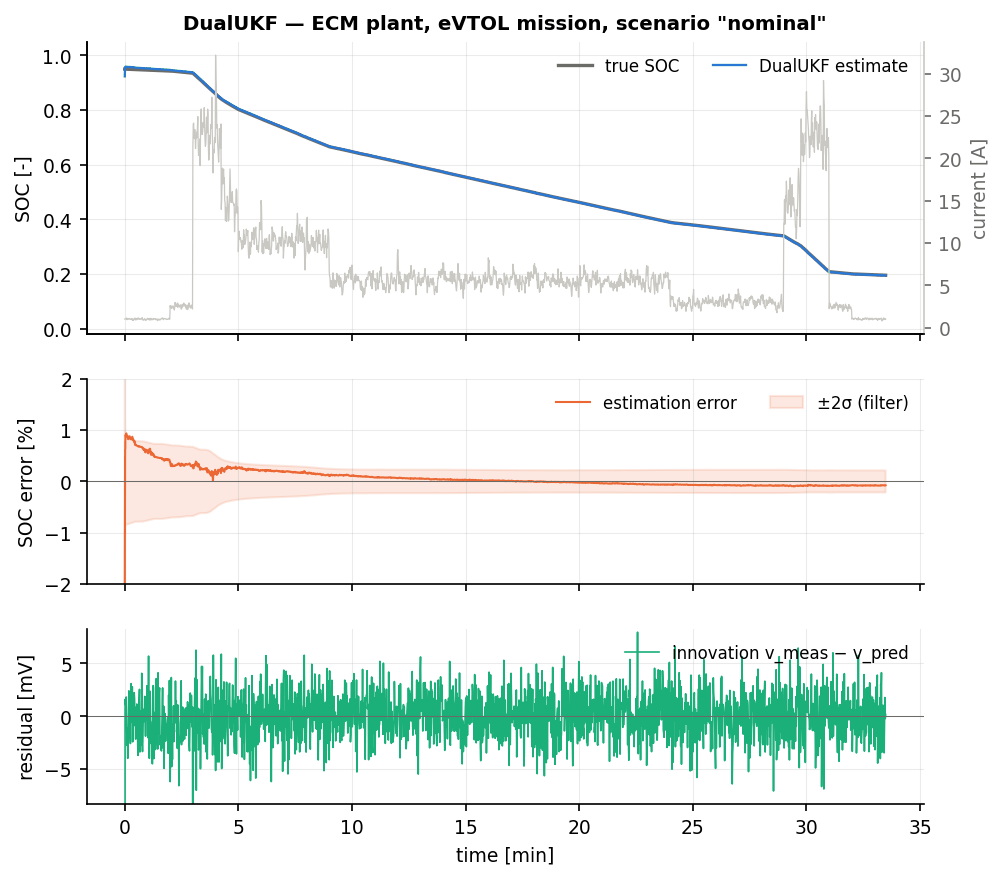
\includegraphics[width=\textwidth]{figures/cell_DualUKF_nominal.png}
\caption{DualUKF on the nominal eVTOL mission: true and estimated SOC (top), estimation error with the $\pm 2\sigma$ band (middle), voltage residual (bottom).}
\end{figure}
\begin{figure}[H]\centering
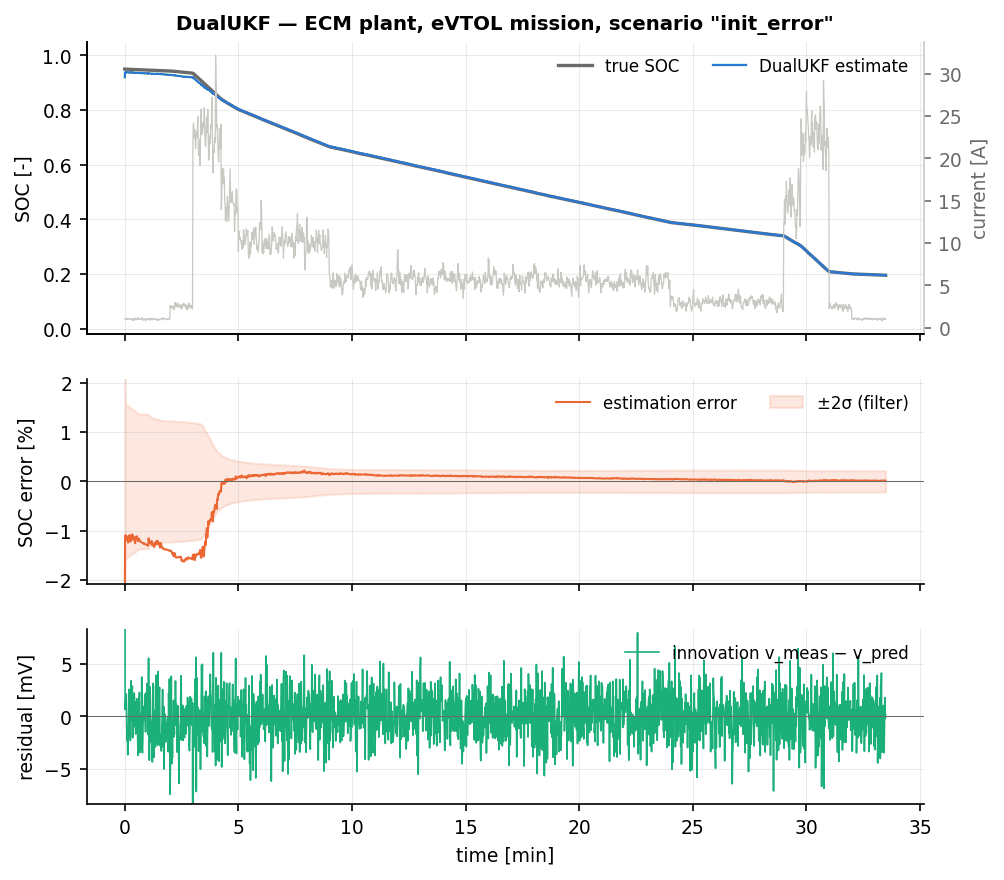
\includegraphics[width=\textwidth]{figures/cell_DualUKF_init_error.png}
\caption{DualUKF with a \SI{35}{\percent} initial SOC error.}
\end{figure}

All figures below are means over three seeds on the eVTOL profile.  On \texttt{nominal} the dual
SPKF reaches $\text{RMSE}=0.0020$ and $\text{RMSE}_\text{ss}=0.0009$, converging at
$t=\SI{0.5}{\second}$; the plain EKF and UKF measured in the same run give $0.0015/0.0005$ and
$0.0020/0.0004$.  On \texttt{init\_error} it reaches $0.0063/0.0012$, but its convergence time is
strongly seed-dependent (\SI{70}{\second} on average over three seeds, against the joint SPKF's
\SI{128}{\second}).  No scenario diverges in any seed.

On \texttt{aged\_cell} it is the best single-flight capacity estimator in the family:
$\texttt{capacity\_err\_end}=\SI{+0.013}{\ampere\hour}$, i.e.\ about \SI{4.25}{\ampere\hour}
recovered from a true \SI{4.23}{\ampere\hour} (\SI{0.3}{\percent} of nameplate), with
$\text{RMSE}_\text{ss}=0.0011$ against the plain EKF's $0.0152$.  The three reference figures:
\begin{center}
\begin{tabular}{@{}lrr@{}}
\toprule
Scenario & $Q_\text{true}$ (\si{\ampere\hour}) & \texttt{capacity\_err\_end} (\si{\ampere\hour})\\
\midrule
\texttt{nominal}      & 5.00 & $+0.029$\\
\texttt{aged\_cell}   & 4.25 & $+0.013$\\
\texttt{current\_bias}& 5.00 & $+0.329$\\
\bottomrule
\end{tabular}
\end{center}
The four joint/dual filters again agree on the \texttt{current\_bias} figure to within
\SI{25}{\milli\ampere\hour} of each other, confirming that it measures the unidentifiability of
$(\alpha,Q)$~\cite{zhao2017observability,lin2018sensorbias} and not an implementation defect.

The scenarios in which the dual SPKF underperforms are \texttt{sensor\_dropout}
($\text{RMSE}_\text{ss}=0.0412$, $\texttt{capacity\_err\_end}=\SI{+0.512}{\ampere\hour}$, the worst
column of the family) and \texttt{param\_mismatch} ($0.0270$, \SI{+0.324}{\ampere\hour}).  Both are
the coloured-residual failure mode: a stuck voltage for \SI{15}{\second} at \SI{22}{\ampere}, or a
persistently wrong $R_1$, produce a residual with a systematic sign that the replica mechanism
cannot cancel because it is genuinely not explained by the state.  The remedy is the same as for the
other dual filter --- robustify the residual, or gate on a quantity that distinguishes model error
from a sensor fault --- and is outside the scope of this chapter.  \texttt{cold} is a third weak column ($0.0161$, \SI{+0.085}{\ampere\hour}): when the time
constants stretch by $3.8\times$ the replica bank, corrected with the state filter's gain, lags the
slower dynamics, and the \emph{fixed} $\gamma_\theta=9$ inflation is then the wrong amount.  That is
the argument for replacing it with the innovation-based adaptive floor the dual EKF uses
(Chapter~\ref{ch:dualekf}, Section~\ref{sec:de-adapt}); the two mechanisms are compatible and the
combination is the obvious next step for this estimator.

\paragraph{The electrochemical plant.}  On the SPM plant the dual SPKF reaches
$\text{RMSE}_\text{ss}=0.0368$ on \texttt{nominal}, essentially level with the plain EKF's $0.0373$
and the plain UKF's $0.0396$: it neither gains nor loses from the structured model error.  That is
already far better than an \emph{unprotected} dual filter manages ($0.1167$ for the dual EKF without
its adaptive floor) --- the fixed $\gamma_\theta=9$ inflation does throttle the parameter filter ---
but well short of the adaptive floor's $0.0086$, which is the quantitative case for adopting it here
too.

\paragraph{Multi-flight capacity tracking.}  Over the 120-flight ageing study
(\texttt{bench\_soh --flights 120 --accel 3}) it tracks the fading capacity with an RMSE of
\SI{33}{\milli\ampere\hour} and a final error of \SI{+22}{\milli\ampere\hour}, the least accurate of
the four joint/dual filters but within \SI{8}{\milli\ampere\hour} of the best.

Cost: \SI{2.38}{\micro\second}/step and \SI{5512}{\byte}.

\section{Summary}
With the state-replica recursion and a $3\sigma$ inflation of the parameter-filter measurement
noise, the dual SPKF is the most accurate single-flight capacity estimator of the four joint/dual
methods (\SI{0.013}{\ampere\hour} on the aged cell), at half the cost of the joint SPKF.  Use it when both capacity and resistance must be
tracked on a temperature-varying mission and the parameter count is large enough that a joint filter
becomes expensive.  Do not implement it with a single shared state estimate: the one-step output
sensitivity to $R_0$ is orders of magnitude larger than the total sensitivity, and the filter will
saturate the resistance within seconds.  Like every dual method it should be paired with a robust
residual test before it is exposed to real sensor faults --- and its fixed noise inflation should be
replaced by the adaptive one of Chapter~\ref{ch:dualekf}, which is what makes the extended dual
filter the best estimator in the benchmark on the electrochemical plant while this one only matches
a plain EKF there.
